		\chapter{RF Networking}
        	\index{RF}
            \index{RF networking}
			Early on in the development of the system I recognized the advantage to having each MCU in the system linked. The primary option was to use RF.
			
			This RF system would be used to start the routine, sync the robots, and aid in the laser localization.
						
			\section{433MHz}	
            	\index{433MHz}
				The first RF solution I experimented with was cheap 433MHz modules that you see riddled all throughout eBay. I happened to buy my \href{http://goo.gl/1zUzJe}\index{transmitter}\index{receiver}{\textit{Transmitter}} and \href{http://goo.gl/pRp4Pb}{\textit{Reciever}} from \index{Jaycar}Jaycar.\\
				
				After playing around for a little while with no success, I posed my problems on the \index{Parallax}\index{forums}\index{Parallax Forums}Parallax Forums.\\
				
				\url{http://forums.parallax.com/discussion/160707/433mhz-rx-noise}\\
				
				I received incredibly valuable advice, especially from Dr\_Acula. From this advice, I wrote a simple driver for the \index{Propeller Chip}Propeller Chip, the code of which can be found here:\\
				
				\url{https://github.com/boar401s2/JaycarTXRX}	
															
				\centerline{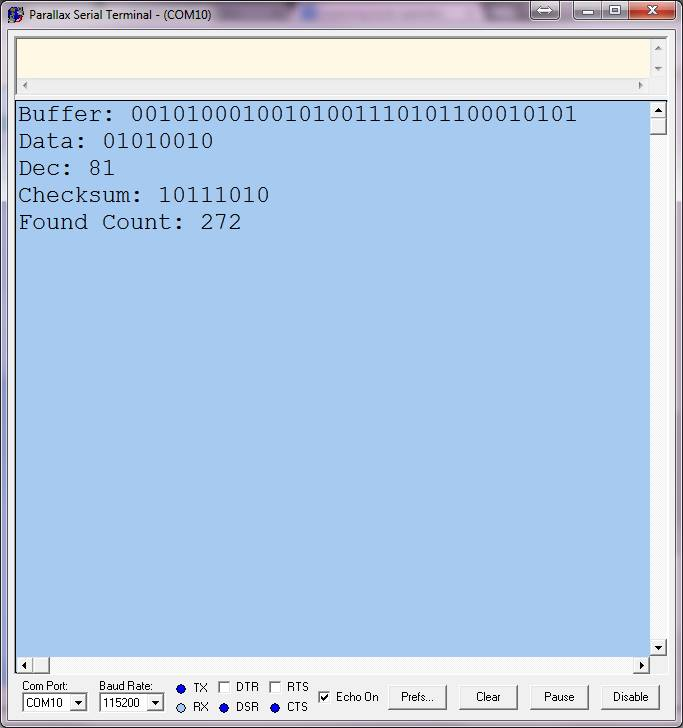
\includegraphics[width=0.75\linewidth]{images/433mhz}}
				
			\section{2.4GHz - nRF24L01+}
            	\label{sec:nRF24L01+}
				Whilst I was working on the 433MHz transmitters, I had also decided to order some nRF24L01+ modules, to also experiment with - and see which were better.\\
				
				I spent a few days researching the \index{nRF24L01+}nRF24L01+ modules, and then I started to write a driver for them in SPIN. Whilst the driver in a \index{MVP}\index{Minimum Viable Product}MVP state, there's still work that can be done on it. The code can be found here: \\
				
				\url{https://github.com/boar401s2/nRF24L01-Driver}\\
				
				Whilst writing the driver software for the 433MHz and nRF24L01+ modules, I had a Saleae Logic Pro 16 \index{logic analyzer}logic analyzer arrive in the post, which significantly helped speed up the development process, and I've also been learning how to use logic analyzers.\\
				
				\centerline{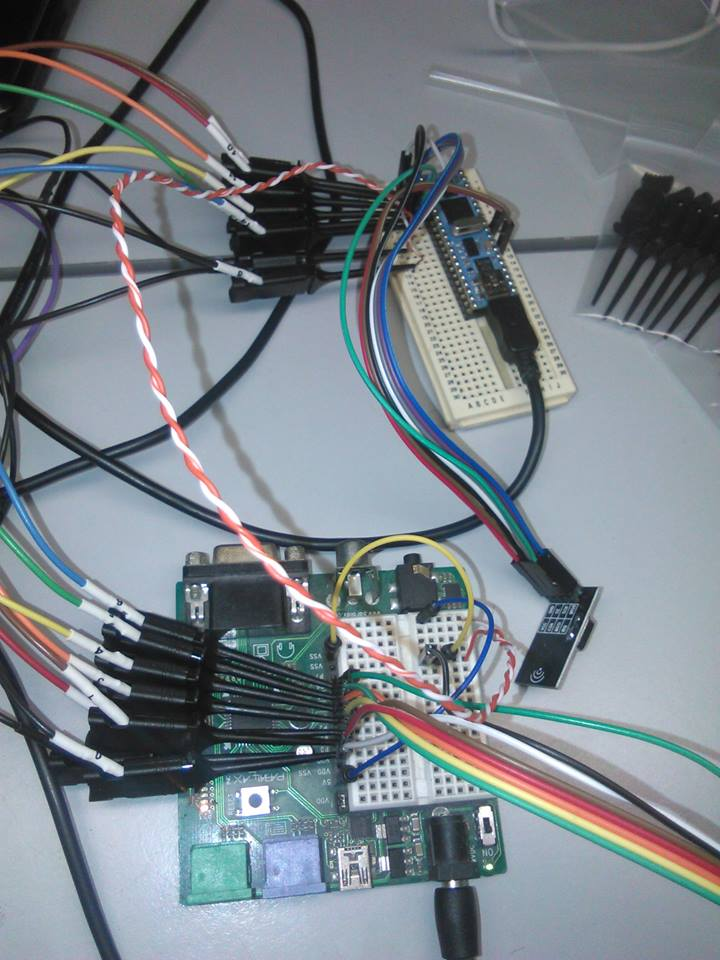
\includegraphics[width=\linewidth]{images/probing_nrf}}				
				\centerline{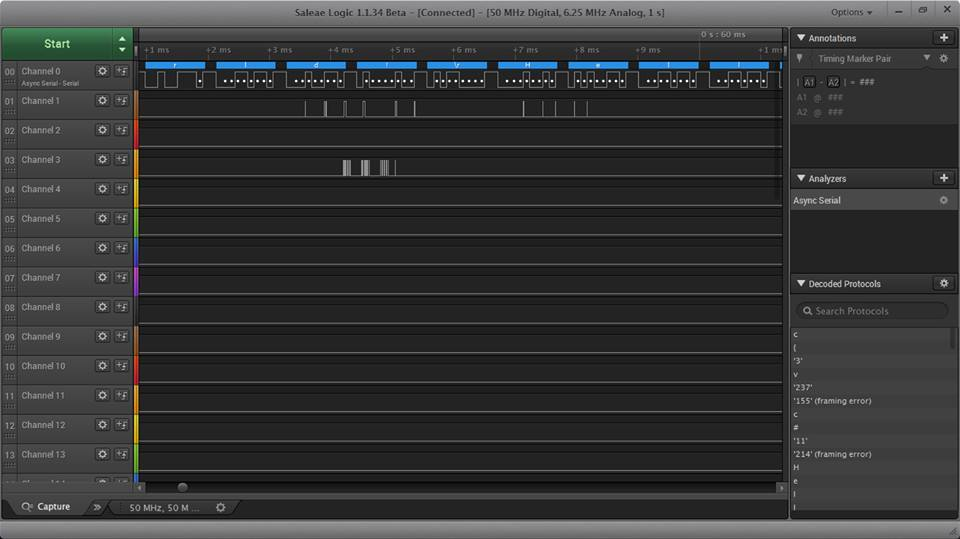
\includegraphics[width=\linewidth]{images/logic_analyser}}
				
				The nature of an event such as RCJA involves lots of laptops/robots using \index{Bluetooth}Bluetooth and/or \index{WiFi}WiFi - which both reside on the RF ISM Band (~2.4GHz). By attempting to implement a network on the 2.4GHz band, foreseeable there could be a lot of interference to contend with.\\
				
				\subsection{2.4GHz interference Solution}
                	\index{solution}
                    \index{}
					Two solutions I came up with was: Use the 433MHz modules, or modulate data signals into the lasers in the Laser Localization System (Personally my favourite solution, although it has many shortcomings!).\\
					
					There is a third option - and that is using IR to communicate - of course this could potentially break the rules as it may interfere with other robots (such as the soccer robots).\\
